\section{Results}
\label{section:results}

%TODO it works better to have this as part of the analysis chapter

%TODO 7.1 belongs to 6.4 .the actual result is simply the number of events in data and the confrontation with the background prediction

As shown in section \ref{sec:bgestimation} $\epsilon^{QCD}_{VBF}$ is calculated for OS ans LS. Uncertainties coming from the stability studies on MC shown in section \ref{dihad:subsec:stability} has been taken into account. The weighted average mean coming from the two different measurements gives the following final result:

\begin{equation}
\epsilon^{QCD}_{VBF} = 0.067\pm0.0046(stat.)^{-0.00038(MC)+0.0117(\tau iso)+0.0056(MET)}_{+0.00022(MC)-0.0051(\tau iso)+0.0022(MET)}
\label{eq:vbfefflsresult}
\end{equation}

Using the following efficiency in Equation \ref{eq:qcdbgpred} gives the final QCD background prediction in signal region:

\begin{equation}
N^{QCD}_{SR} = 7.14\pm0.92(stat.)^{-0.42(MC)+1.34(\tau iso)+0.64(MET)}_{+0.35(MC)-0.58(\tau iso)+0.25(MET)}
\label{eq:QCDbgpredresult}
\end{equation}

This final estimate is corrected for the MET bias by taking the central value of the  bias as a correction and 
the uncertainty of the central value as a symmetric uncertainty. The result of this correction is shown in Eq.
\ref{dihad:eq:QCDbgpredCorrectResult}

\begin{equation}
N^{QCD}_{SR} = 7.59\pm0.92(stat.)^{-0.42(MC)+1.34(\tau iso)+0.20(MET)}_{+0.35(MC)-0.58(\tau iso)-0.20(MET)}
\label{dihad:eq:QCDbgpredCorrectResult}
\end{equation}

\section{Final Yields for LS channel}

%TODO that implies that di-tau charge requirement is not part of event selection. is that intentional?

%TODO "QCD is the dominant background....: weird sentence the table should contain a number “total background” to be compared with the data."

%TODO "A good agreement in all ..." : here you need to mention that the statistics is really low. a meaningful comparison data to bkg prediction is not really possible

The like-sign signal region consist of events satisfying the criteria shown in section \ref{sec:eventselection} with the di-$\tau$ charge requirement. As described in section \ref{dihad:subsubsec:eventweight} all the backgrounds have been reweighted with $\tau_{h}^{fake}$ reweighting method. Table \ref{table:SReventcount} shows the contributions in the signal region from all MC samples and data.  QCD is the dominant background and its prediction shown in section \ref{section:results} is compatible with the number in table \ref{table:SReventcount}. Figure \ref{fig:LS_SR_h_met_dijetinvariantmass_log}(a) shows the expected and observed signal rate in bins of \met. Figure \ref{fig:LS_SR_h_met_dijetinvariantmass_log}(b) shows the expected and observed signal rate in bins of $M_{jj}$. A good agreement in all the distributions range between observed data and the SM prediction is observed. Additional distributions for signal region have been included in the Appendix.

   \begin{table}[ht]
     \centering{
     
  %   \tabcolsep=0.05cm
      \begin{tabular}{| l | c |}
         \hline\hline
         Sample     &Events (SR)      \\ [0.5ex] \hline
Data &$ 9 $     \\
Drell-Yan &$ 0.037\pm0.015$      \\
VV &$ 0.11\pm0.065$     \\
W+Jets &$ 0.53\pm0.04$        \\
Single t &$ 0.036\pm0.0066$    \\
TTbar &$ 0.11\pm0.012$    \\
Higgs &$ 0.0005\pm7.2e-05$     \\
QCD Prediction &$ 7.59\pm0.92(stat.)^{+1.38}_{-0.72}(syst.)$    \\
\hline
Total nonQCD MC &$ 0.83\pm0.079(stat.)\pm0.41(syst.)$    \\
         \hline\hline
       \end{tabular}
     }
     \caption{\label{table:SReventcount}Number on events in SR data and all MC samples. The QCD prediction has been corrected for the unidirectional MET-bias described in section \ref{dihad:subsec:stability} for the combination of the systematic errors.}
      % is used to refer this table in the text
   \end{table}
   
       \begin{figure}[tbh!]
           \centering
           \begin{tabular}{cc}
             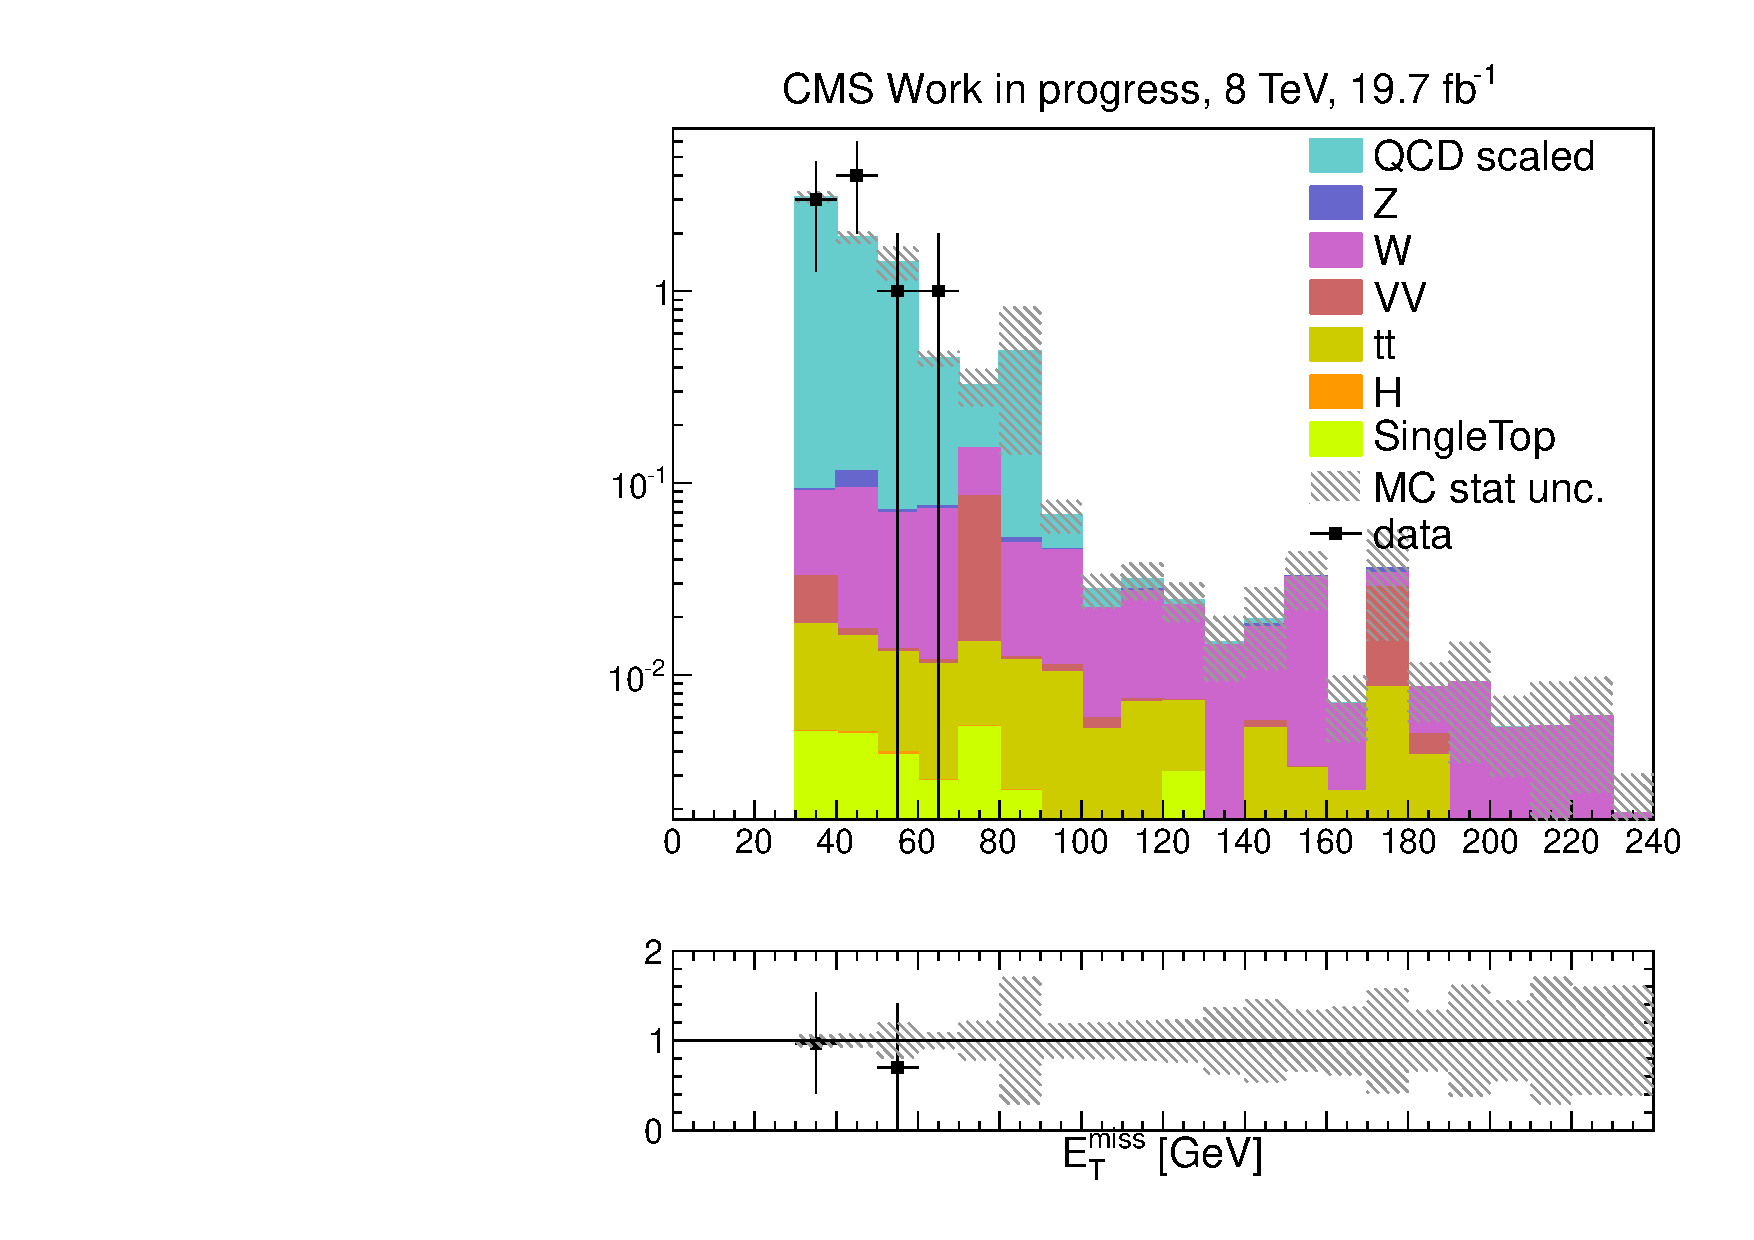
\includegraphics[width=0.40\textwidth]{PLOTS/diTauHadLSQCDPlots/UnblindedUpdate/LS_SR/LS_SignalRegion/h_met_log.pdf}
             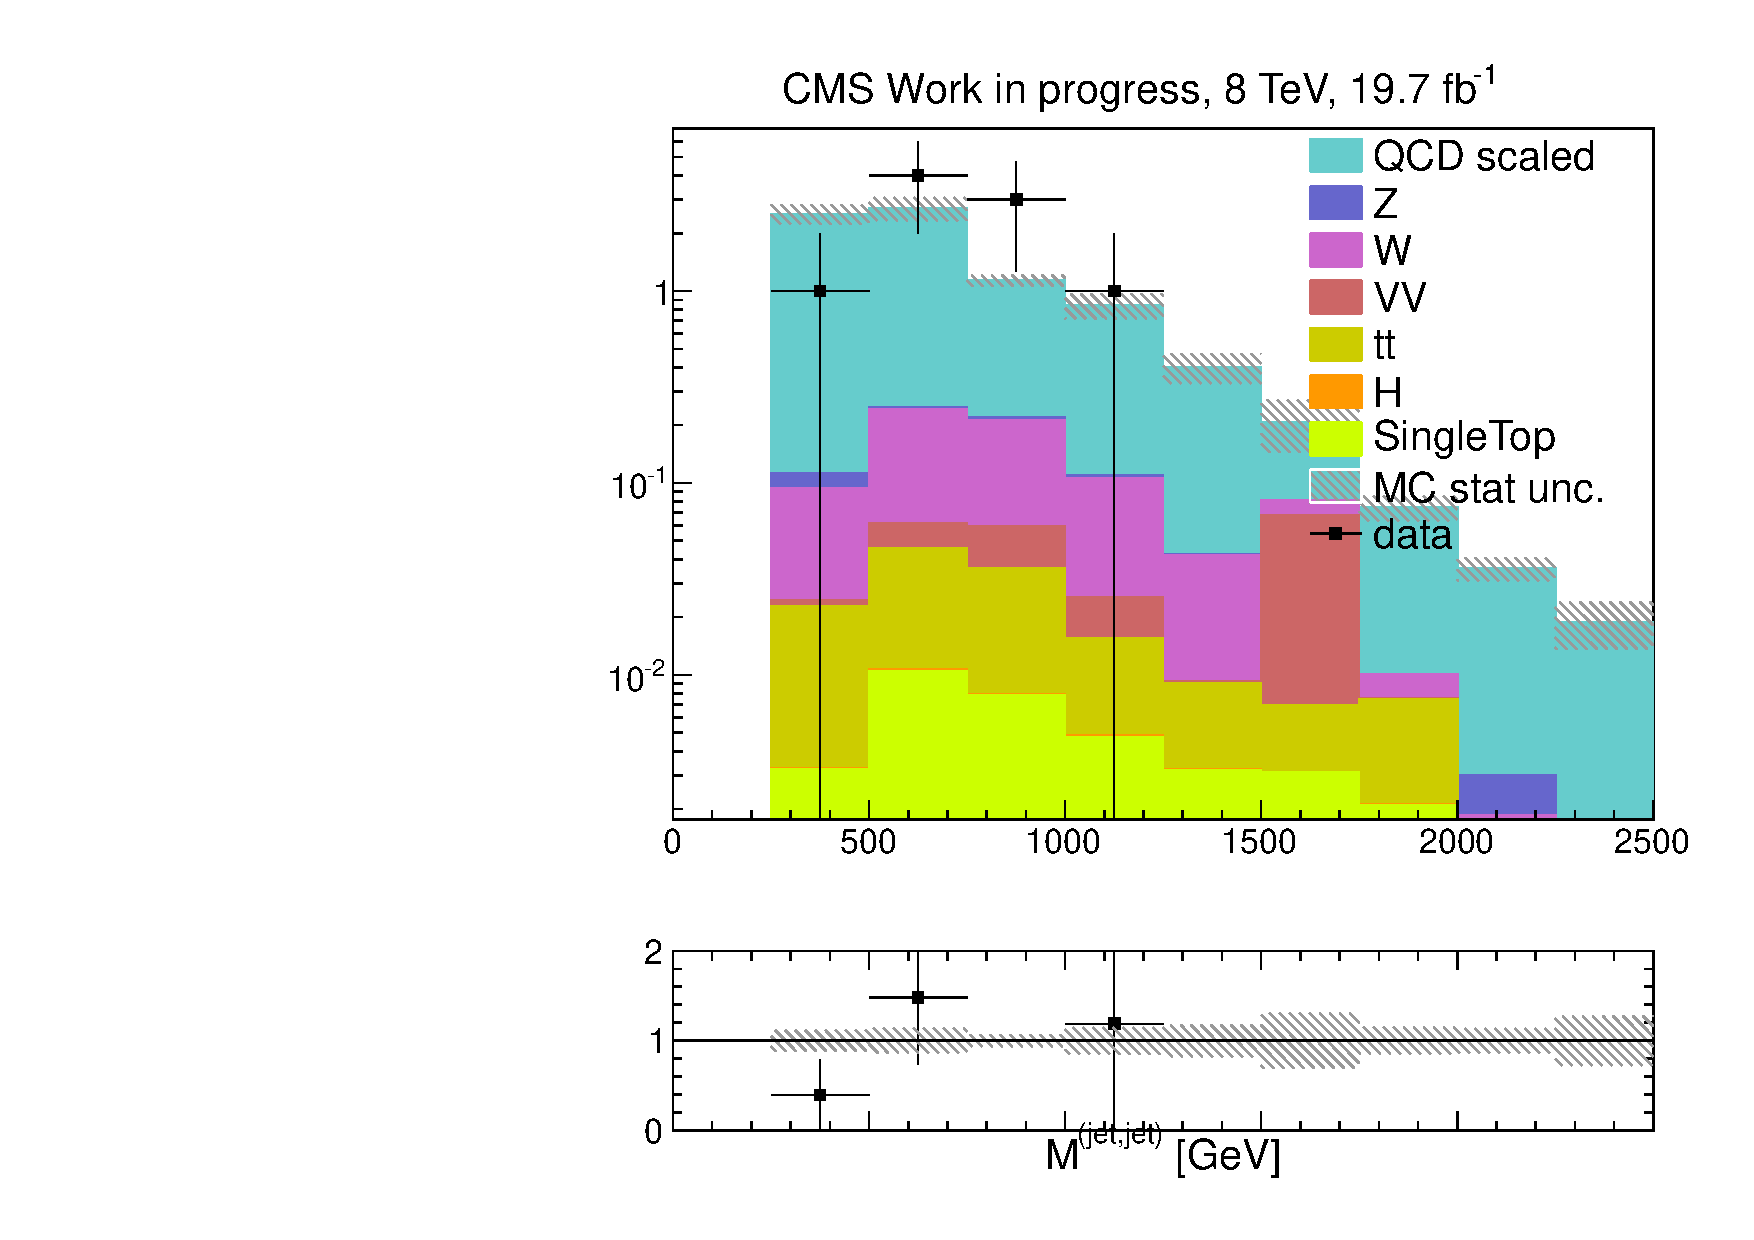
\includegraphics[width=0.40\textwidth]{PLOTS/diTauHadLSQCDPlots/UnblindedUpdate/LS_SR/LS_SignalRegion/h_dijetinvariantmass_log.pdf}
           \end{tabular}
           \caption{(a) \met and (b)$M_{jj}$ distributions in signal region for Data and all MC samples}
           \label{fig:LS_SR_h_met_dijetinvariantmass_log}
         \end{figure}

\clearpage 
\section{Systematics}
\label{sec:systematics}

%TODO systematic uncertainties on what exactly? just signal predictions in signal region? background predictions in signal regions and control regions?

%TODO the analysis chapter needs a section about signal samples, somewhere rather early in the chapter

The following systematics have been considered:

\begin{itemize}
	%TODO which cross section? signal? each possible signal?
  \item \textbf{Parton Distribution Functions (PDF):} The systematic effect due to imprecise knowledge of the parton distribution functions is determined by comparing CTEQ6.6L \cite{Nadolsky:2008zw}, MSTW2008nnlo \cite{Martin:2009iq}, and NNPDF20 PDF \cite{Ubiali:2008uk} with the default PDF and variations within the family of parametrization. The maximal deviation from the central value is used the overall systematic due to PDFs. We obtain a value of 16\% on the cross section uncertainty and 23\% on the signal acceptance.

  \item \textbf{Initial State Radiation (ISR) and Final State Radiation (FSR):} The systematic effect due to imprecise modeling of initial and final state radiation is determined by re-weighting events to account for effects such as missing a terms in the soft-collinear approach \cite{Nanava:2003cg} and missing NLO terms in the parton shower approach \cite{Miu:1998ju}. We obtain uncertainties of 0.9\% and 1.2\% for ISR and FSR respectively.

  \item \textbf{Luminosity:} We consider a 2.6\% uncertainty on the measured luminosity \cite{CMS:2012rua}.
  
  \item \textbf{Trigger, Reconstruction, and Selection:}  An overall uncertainty is applied for the trigger uncertainties determined on the correction factors described in AN-12-321 and which are measured using tag-and-probe methods. We consider 6.8\% uncertainty per hadronic tau leg \cite{CMS:2011msa}. Scale factors for $\tau_{h}$ identification are taken from the tau POG and obtained using a fit of data in a Z$\to\tau\tau$ enhanced region and fixing the cross section to that measured using ee/$\mu\mu$. We consider a 100\% correlation among the 2 tau legs, therefore we consider 13.6\% uncertainty on the signal acceptance.

  \item \textbf{$b$-Tagging Efficiency:} We consider a 30\% uncertainty on the mis-tag rate as measured by the b-tagging POG \cite{CMS:2011cra}. For the case of our signal, the systematic uncertainty on the requirement of 0 jets mis-tagged as b-jets is determined by propagating the 30\% uncertainty on the mis-tag rate through the following equation (which represents the signal efficiency for requiring 0 jets mis-tagged as b-Jets):

\begin{equation}\label{eq:nttbar}
  \epsilon^{\textrm{NBtag} < 1} = 1 - \sum_{n=1} P(n) \cdot \sum_{m=1}^{n} C(n,m) \cdot f^{m} \cdot (1-f)^{n-m}
\end{equation}

where $P(n)$ is the probability to obtain $n$ additional jets (non-tau and non-lepton) in the event, $C(n,m)$ the combinatorial of $n$ $choose$ $m$, and $f$ the mis-tag rate. The probability to obtain at least one additional jet in the event is much less than 1\%. Therefore, based on the above equation, the mis-tag rate and uncertainty, and the probability to obtain at least one additional jet we calculate a negligible systematic effect on our signal due to the mis-tag rate.

  \item \textbf{Tau Energy Scale:} We consider the effect of the 3\% tau energy scale uncertainty measured by the tau POG on the signal acceptance. The tau 4-momentum is scaled by a factor of $k=1.03$ ($p_{smeared} = k \cdot p_{default}$) and variables are recalculated using $p_{smeared}$. We find that by using $p_{smeared}$ calculated with a factor of $k=\pm 1.03$, the signal acceptance fluctuates by 4\%. Therefore, we assign a 4\% systematic on the signal acceptance due to tau energy scale.
  \item \textbf{Jet Energy Scale:}  The uncertainty on jet energy correction (JEC) is the result of a factorized approach on $Anti­-k_{t}$ jets with $R=0.5$ clustered from Particle Flow (PF) candidates. For MC samples JEC is divided in different steps that take into account several levels of correction. The fist step consist in a single level of corrections (L1) which estimates the $p_{t}$ offset in bins of $\eta$ and $N_{PV}$ for AK5PF jets. The second step, known as MC-Truth Corrections, consists in two level of corrections (L2 and L3) converging into an $\eta$ , $p_{t}$ ­dependent scaling factor fully derived from MC after applying L1­ corrections. The last step takes into account an L5 correction and uncertainties for individual flavors and predefined mixtures inside the reconstructed jets. We assign a 2\% systematic on the signal acceptance due to jet energy scale.
  \item \textbf{Jet Energy Resolution:}  The measured jet transverse momentum is not necessarily equal to the energy of the original particle due to e.g. a limited detector resolution. This effect is quantified by the jet transverse momentum response R which is defined as $R = p_{T} / p_{T}^{particle}$  where $p_{T}$ denotes the transverse momentum of the jet measured at detector level and $p_{T}^{particle}$ is the transverse momentum of the original particle-level jet. The average response $\langle R \rangle$ is referred to as jet energy scale and calibrated such that $\langle R \rangle = 1$ for fixed $p_{T}^{particle}$. The response usually depends on the jet momenta as well as on the pseudorapidity. This is expected since the quality of the jet measurement is directly related to the detector sub-components and the energy of the particles originating e.g. from the track-reconstruction efficiency or the individual amount of detector material. The core of the response is caused by the intrinsic resolution of the various sub-detector components and the precision of the jet clustering algorithms. The response tails are mainly caused by severe jet-mismeasurements. These can be e.g. detector effects like shower leakage or detector noise. Finally, the relative jet transverse momentum resolution is defined as the width of the response distribution corresponding to the gaussian part and hence is a function of $p_{T}$ and $\eta$ as well as the total response. One possibility to measure the resolution of the jet transverse momenta in data as well as in simulated events is to utilize the dijet asymmetry A. For events with at least two jets it is defined as:
  
  \begin{equation}
  A = \frac{p_{T,1} - p_{T,2}}{p_{T,1} + p_{T,2}}
  \end{equation}
  
  For a sufficient number of events the asymmetry is approximately normally distributed and its standard deviation is $\sigma_{A}$. In an ideal dijet topology the two jets are exactly balanced at particle level which leads to an important relation between the width of the asymmetry $\sigma_{A}$ and the jet-$p_{T}$ resolution $\sigma(p_{T})$:
  
  \begin{equation}
  \frac{\sigma(p_{T})}{\langle p_{T} \rangle} = \sqrt{2} \sigma_{A}
  \end{equation}
  
  Using the latest JER uncertainty collection from \texttt{Summer13\_\-V5\_DATA\_\-Uncertainty\-Sources\_\-AK5PFchs.txt} assign a 4\% systematic on the signal acceptance due to jet energy resolution. 

  \item \textbf{MET:} The uncertainty on MET for our signal process is driven by the jet energy scale (non-tau jets) (JES), light lepton energy/momentum scale (LES), and unclustered energy (UCE). The systematic effect from MET due to TES, JES and LES is included in the JES, TES, LES systematic uncertainties described above. We find that a 10\% uncertainty on the unclustered energy resultsin at most a 0.5\% fluctuation on the signal acceptance.
\end{itemize}

\begin{table}[h]
	\centering{
		\begin{tabular}{| l | c | c |}
			\hline\hline
			Source            & Uncertainty & Signal \\
			\hline
			PDF               & ---                            & 23\%                       \\
			ISR/FSR           & ---                             & 1\%              \\
			Luminosity        & 2.6\%                           & 2.6\%                      \\
			Trigger, ID, Selection & 6.8\%                            & 16\%                       \\
			Tau Energy Scale  & --                             & 4\%                        \\
			b-Jet ID          & 30\%                            & 1\%                        \\
			JES               & 2\% - 10 \%                            & 2\%                      \\
			JER              & 5\% - 25 \%                            & 4\%                      \\
			MET               & 10\%                           & 0.5\%  \\
			\hline\hline                  
			\end{tabular}
	}
\caption{Summary of systematic uncertainties}
\label{table:Uncertainties}
\end{table}

Table \ref{table:Uncertainties} summarizes all the relevant uncertainties that has been considered. 

\clearpage

\section{Limits}

%TODO i recommend one additional section “combined results” at the very end of the analysis chapter, where you provide an overview of the results of all channels and show the limits for the combination of all results

Upper limits at $95\%$ on the cross sections as function of $m_{\tilde{\chi}_{2}^{0}}=m_{\tilde{\chi}_{1}^{\pm}}$ are set for LS and OS channel. The results are presented using models with a fixed mass for the LSP $m_{\tilde{\chi}_{1}^{0}} = 0 $ GeV, a $\tilde{\chi}_{1}^{\pm}$ mass between $100 \leq m_{\tilde{\chi}_{1}^{\pm}} \leq 300$ GeV and a $\tilde{\tau}$ mass of $m_{\tilde{\tau}} = 0.95 m_{\tilde{\chi}_{1}^{\pm}}$ .

\begin{figure}
  \begin{center}
    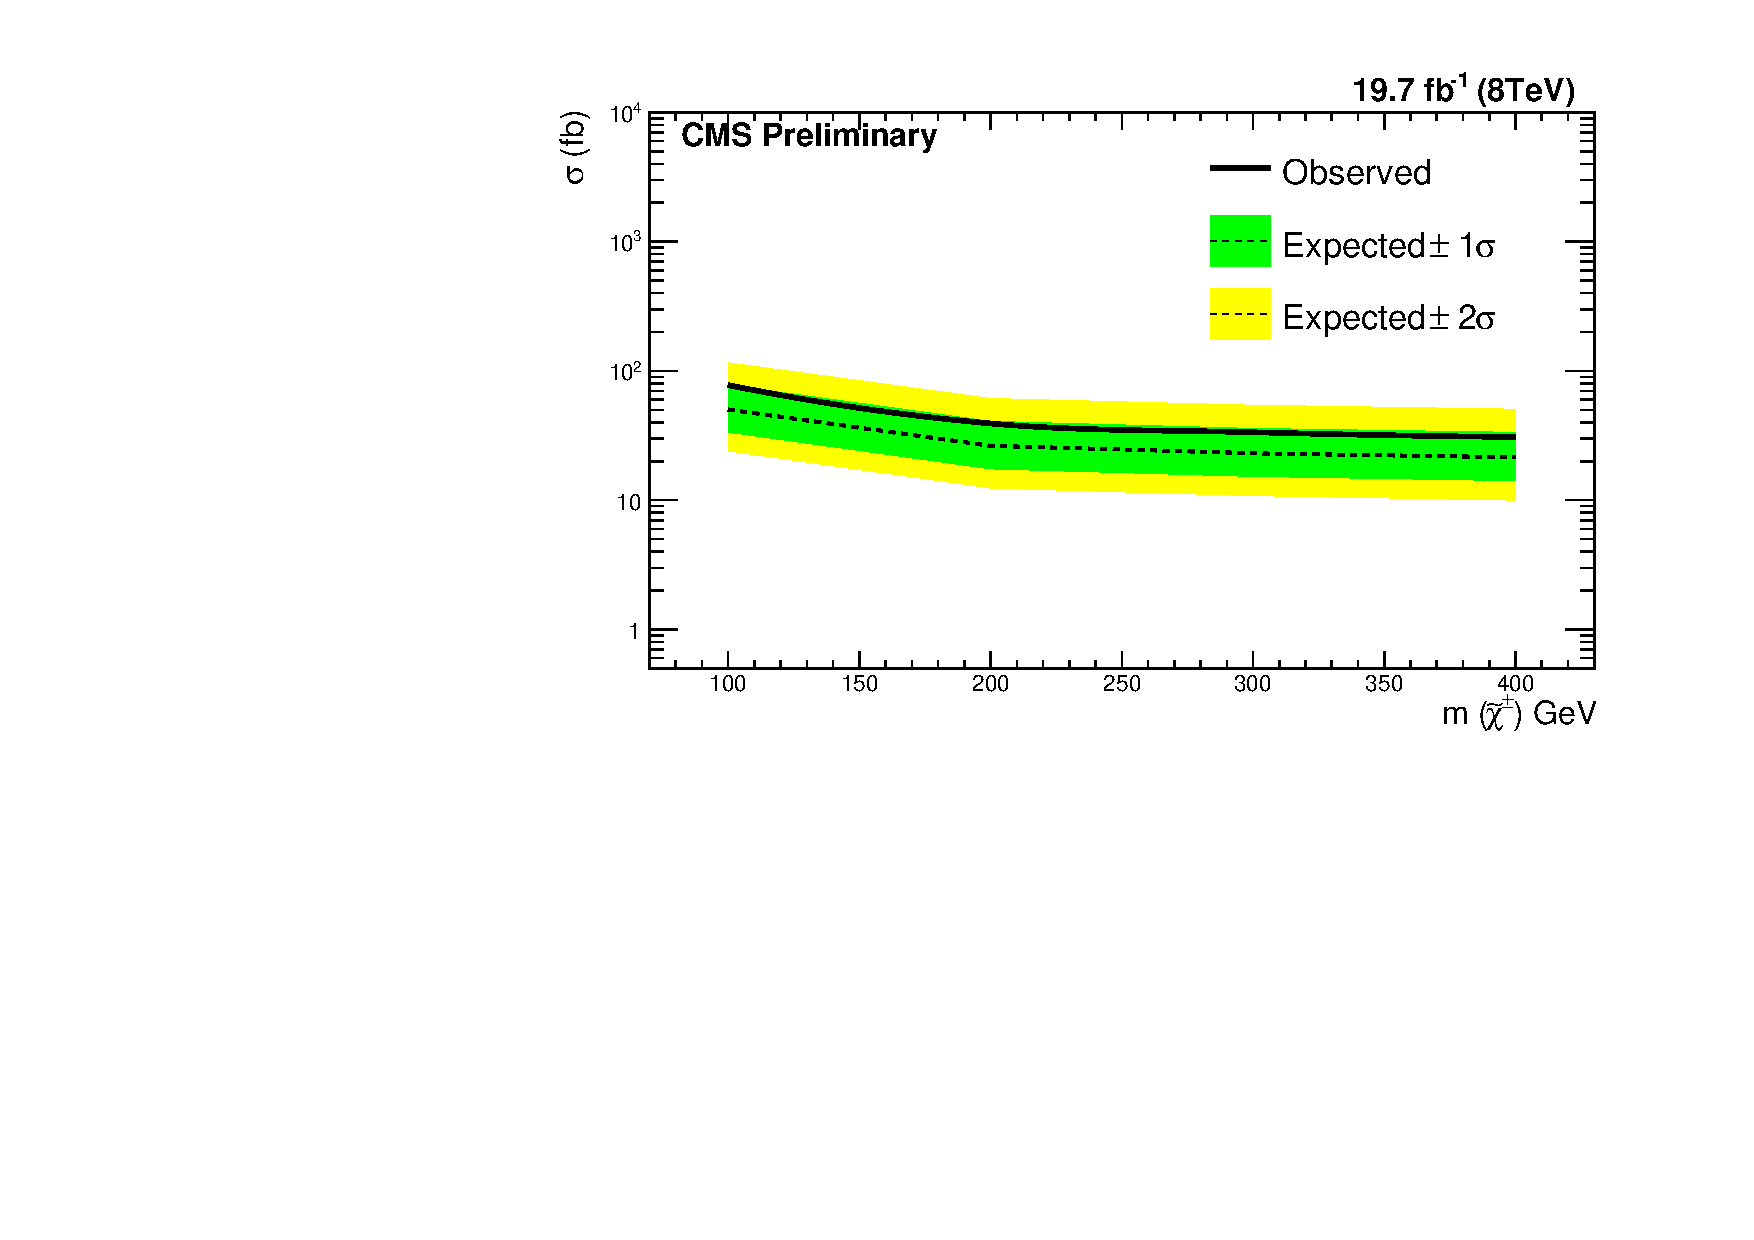
\includegraphics[angle=0,width=.48\textwidth, height=0.35\textheight]{PLOTS/Limit_VBF_diTau_OS.pdf}
    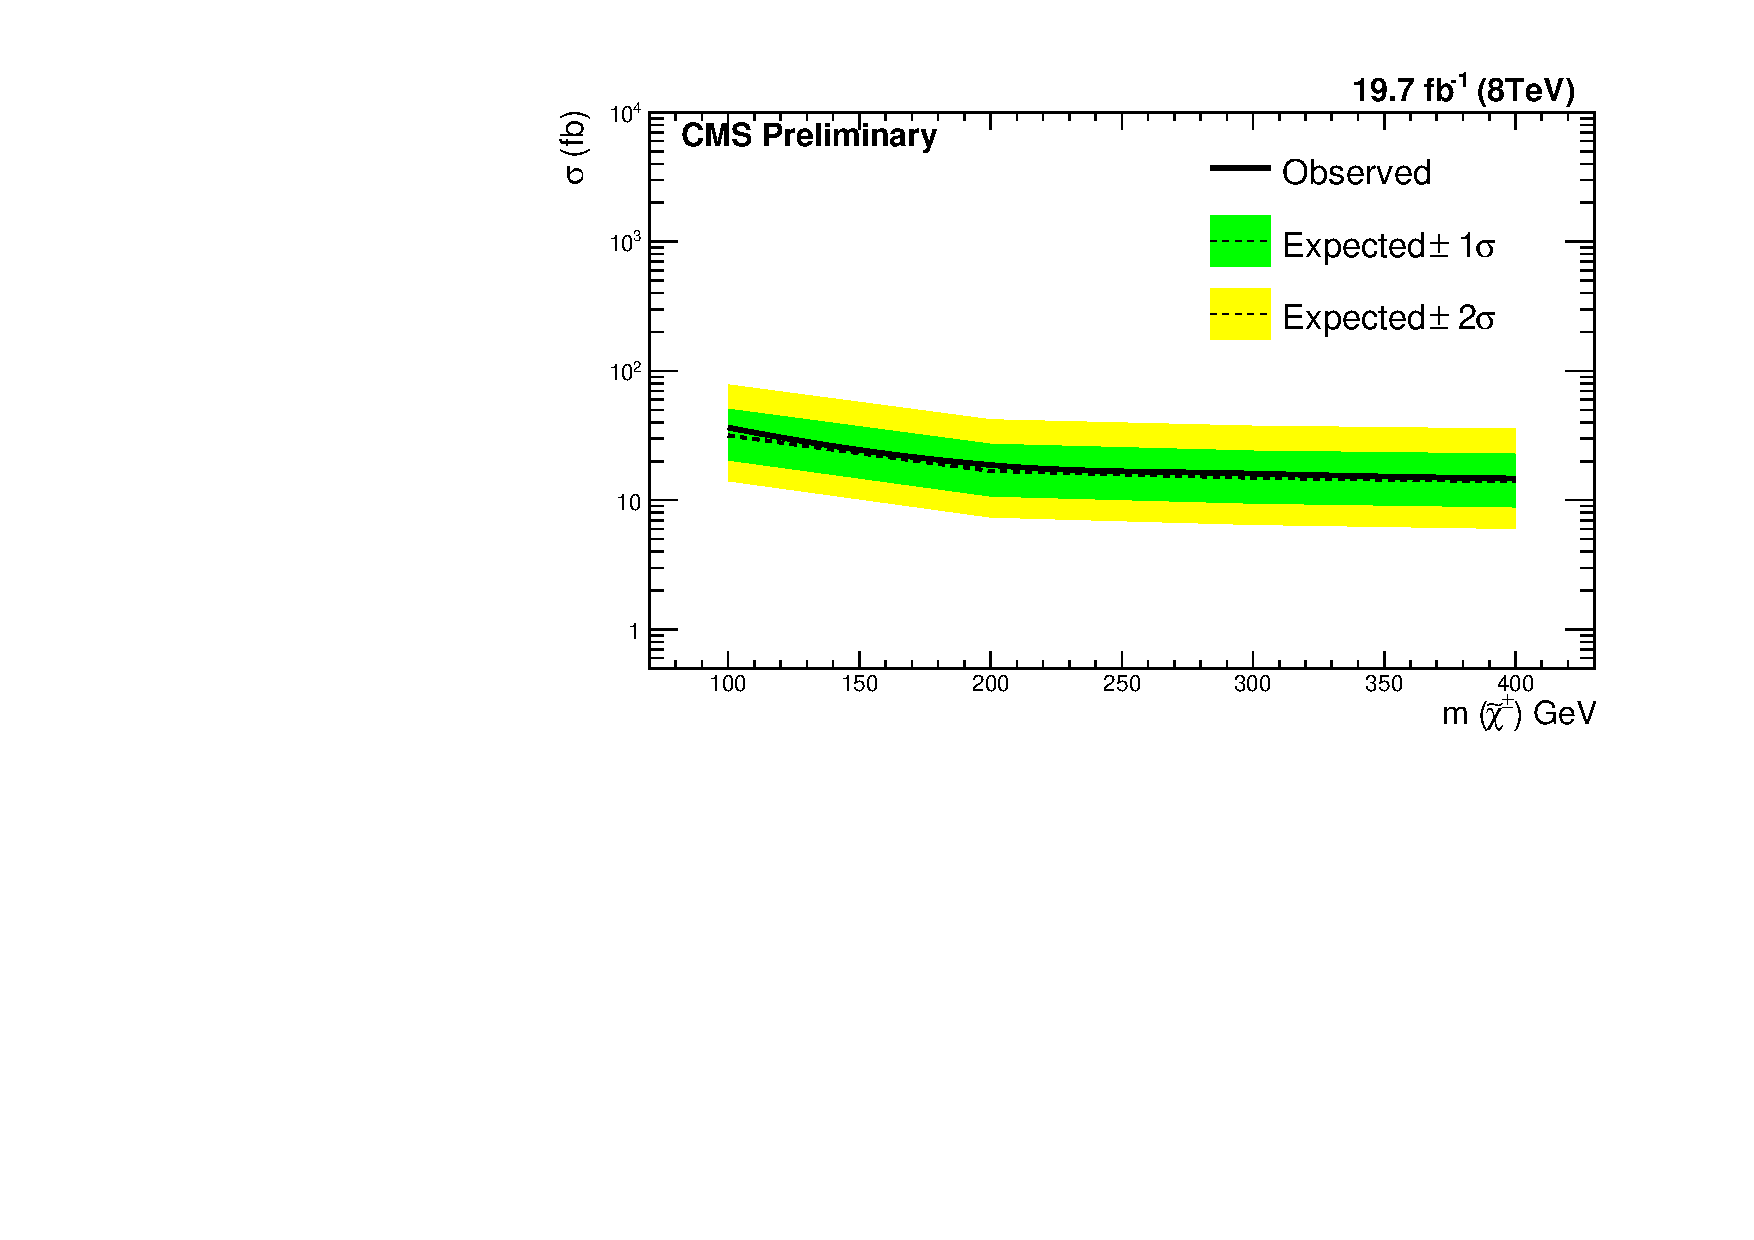
\includegraphics[angle=0,width=.48\textwidth, height=0.35\textheight]{PLOTS/Limit_VBF_diTau_LS.pdf}
    \caption{Upper limit at the 95\% CL on the cross-section as a function of 
$m_{\tilde{\chi}_{2}^{0}}=m_{\tilde{\chi}_{1}^{\pm}}$ for the (a) OS 
$\tau_{h}\tau_{h} j_{f} j_{f}$, (b) LS $\tau_{h}\tau_{h} j_{f} j_{f}$
final states. The bands represent the one and two standard deviations obtained from the background-only hypothesis.}
  \label{fig:LimitsOSLS}
 \end{center}
\end{figure}

\begin{figure}
  \begin{center}
    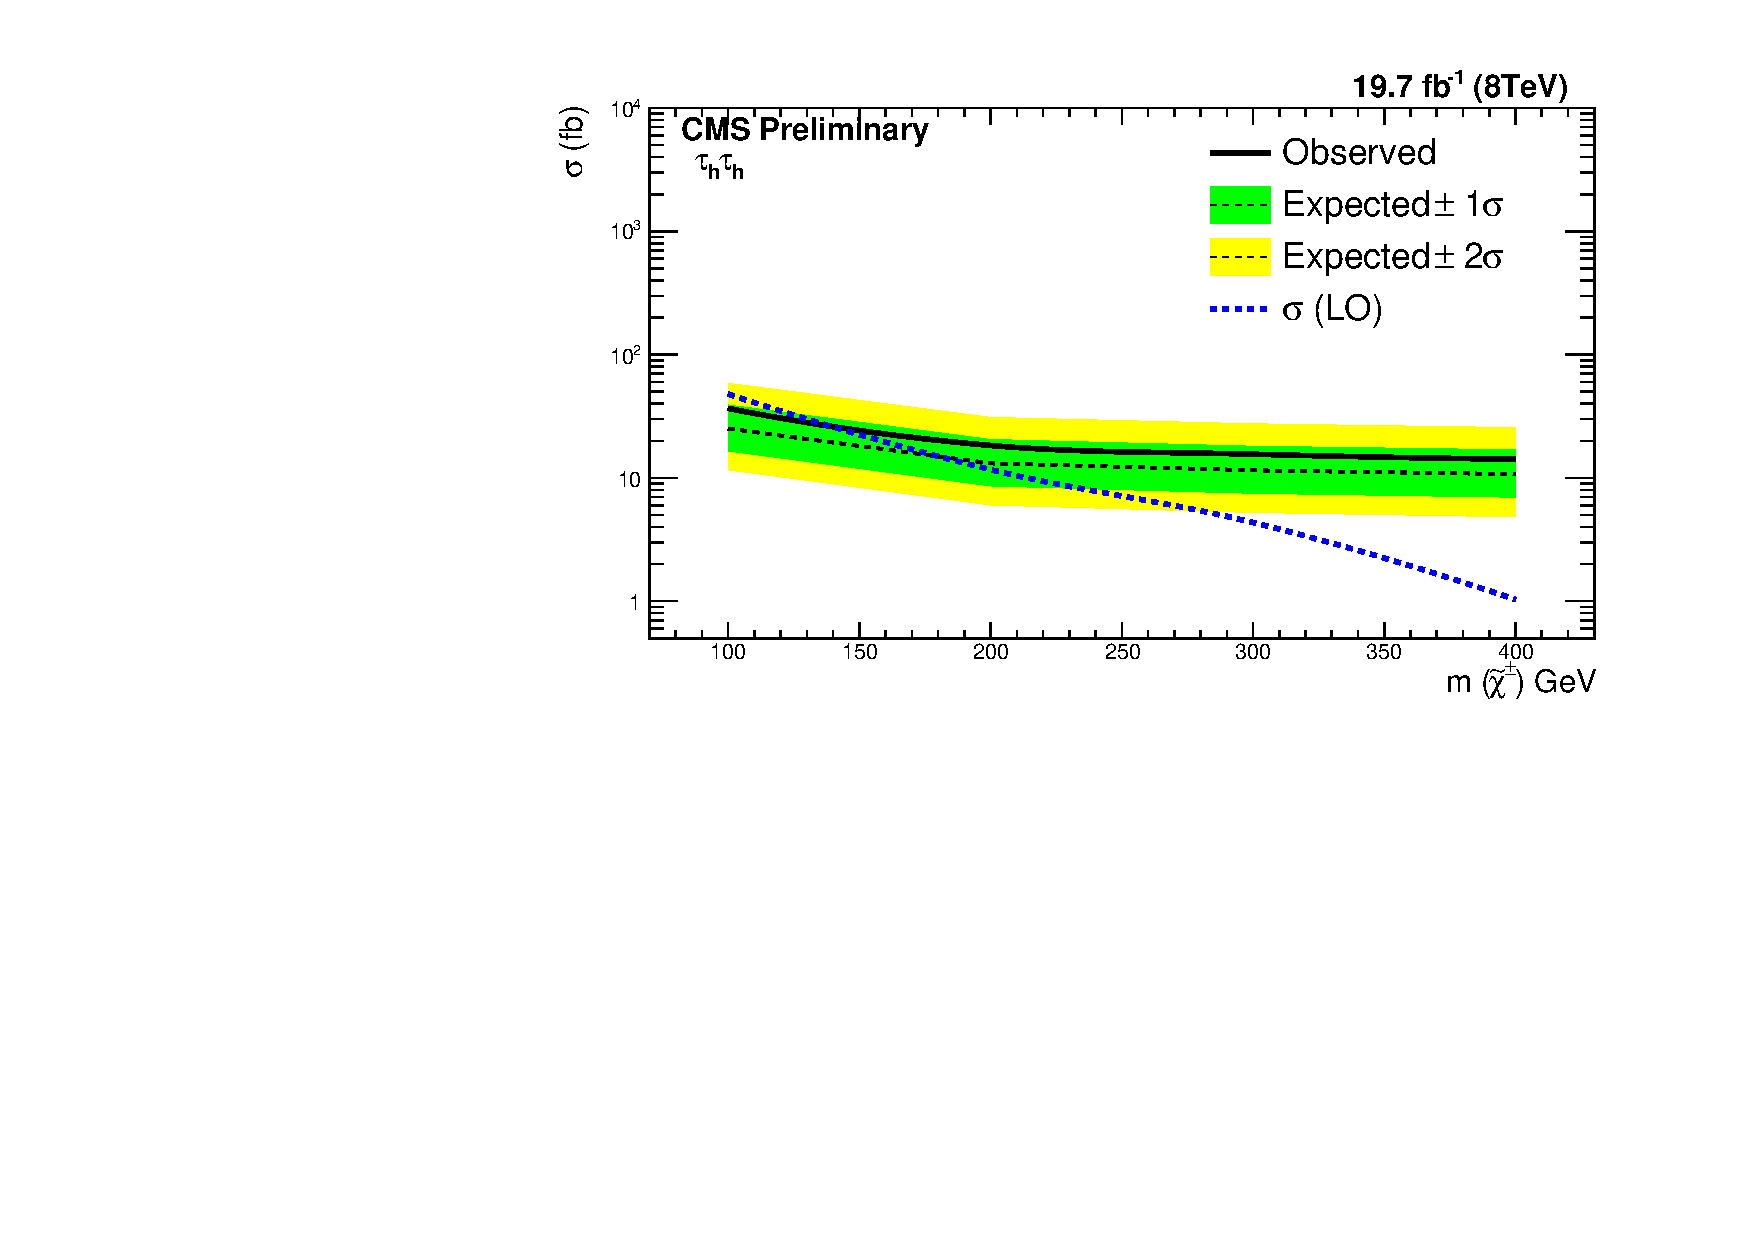
\includegraphics[angle=0,scale=0.75]{PLOTS/Limit_VBF_diTau_combined.pdf}
    \caption{Upper limit at the 95\% CL on the cross-section as a function of 
$m_{\tilde{\chi}_{2}^{0}}=m_{\tilde{\chi}_{1}^{\pm}}$ for the combination of OS and LS $\tau_{h}\tau_{h} j_{f} j_{f}$
final states. The bands represent the one and two standard deviations obtained from the background-only hypothesis.}
    \label{fig:LimitsCombination}
 \end{center}
\end{figure}

Figure \ref{fig:LimitsOSLS}(a) \ref{fig:LimitsOSLS}(b) and  shows the upper limit at the 95\% CL on the cross-section for OS and LS channel. A combination of the two channels is shown on Figure \ref{fig:LimitsCombination}. The upper expected limit on $m_{\tilde{\chi}}$ corresponds to the point where the expected limit crosses the theoretical line and is set for  $\tilde{\chi}_{1}^{\pm} /\tilde{\chi}_{2}^{0} $ with masses of 180 GeV. The upper observed limit on $m_{\tilde{\chi}}$ corresponds to the point where the observed limit crosses the theoretical line. We exclude $\tilde{\chi}_{1}^{\pm} /\tilde{\chi}_{2}^{0} $ with masses below 140 GeV in the models considered. The limit results coming from OS and LS $\tau_{h}\tau_{h} j_{f} j_{f}$ final states are combined with other 6 channels documented on AN-12-321 for the final upper limit.


